
\documentclass[12pt]{article}

\usepackage[utf8]{inputenc}
\usepackage[greek, english]{babel}

% Packages

\usepackage{alphabeta}
\usepackage{amsmath}
\usepackage{amsthm}
\usepackage{caption}
\usepackage{color}
\usepackage{fullpage}
\usepackage{graphicx}
\usepackage{latexsym}
\usepackage{listings}
\usepackage{pxfonts}
\usepackage{stackrel}
\usepackage{titlesec}

% Commands
\newcommand{\R}{\mathbb{R}}
\newcommand{\N}{\mathbb{N}}
\newcommand{\norm}[1]{\left\lVert#1\right\rVert}
\newcommand{\margin}{\hspace{4pt}}
\newcommand{\centered}[1]{\begin{align*}#1\end{align*}}
\newcommand{\plot}[2]{\includegraphics{#1}\caption{#2}}
\newcommand{\code}[2]{\lstinputlisting[caption={#2}]{#1}}

% Environments
\newenvironment{rcases}
	{\left.\begin{aligned}}
	{\end{aligned}\right\rbrace}

\newenvironment{matlab}
	{\begin{figure}[hp]\centering\captionsetup{justification=centering}}
	{\end{figure}}

% Python Syntax Highlighting
\definecolor{string_color}{RGB}{0, 161, 13}
\definecolor{comment_color}{RGB}{46, 46, 46}
\definecolor{keyword_color}{RGB}{0, 112, 191}

\lstset{
    language=Python,
    captionpos=b,
    numbers=right,
    numberstyle=\small\ttfamily,
    frame=lines,
    showspaces=false,
    showtabs=false,
    breaklines=true,
    showstringspaces=false,
    breakatwhitespace=true,
    commentstyle=\color{comment_color}\textit,
    keywordstyle=\bfseries\color{keyword_color}\textbf,
    stringstyle=\color{string_color}\textit,
    morekeywords={self, lambda, __init__, __del__, __name__, for, in, not, and, or, :},
    basicstyle=\ttfamily,
    tabsize=4,
    keepspaces=true,
    columns=flexible
}

% Lengths
\setlength{\parindent}{0in}
\setlength{\oddsidemargin}{0in}
\setlength{\textwidth}{6.5in}
\setlength{\textheight}{10in}
\setlength{\topmargin}{-1.0in}
\setlength{\headheight}{18pt}

\titlespacing*{\subsection}
{0pt}{5.5ex plus 1ex minus .2ex}{4.3ex plus .2ex}

\title{\hugeΑλγοριθμική Επιχειρησιακή Έρευνα\\Τρίτη Εργασία}
\author{Σιώρος Βασίλειος\\Ανδρινοπούλου Χριστίνα}
\date{Οκτώβριος 2019}

\begin{document}

\maketitle

\pagenumbering{gobble}

\pagebreak


\subsection*{Examples of Linear Programming Problems: Pattern classification}

Έστω ότι έχουμε m αντικείμενα και θέλουμε να τα διαχωρίσουμε σε δύο διακριτές ομάδες. Κάθε αντικέιμενο ανήκει αυστηρά σε μία μόνο ομάδα. \\

Για να το επιτύχουμε αυτό πρέπει να είμαστε σε θέση να περιγράψουμε κάθε αντικείμενο. Επιλέγουμε καθολικά για όλα τα αντικείμενα n το πλήθος χαρακτηριστικά, τα οποία οργανώνουμε σε ένα vector. Συνεπώς, κάθε αντικείμενο περιγράφεται από ένα vector μεγέθους n. \\

Ωστόσο, για να είμαστε σε θέση να μιλάμε για διαχωρισμό των αντικειμένων σε δύο διακριτές ομάδες, θα πρέπει να γνωρίζουμε ότι τα αντικείμενά μας όντως μπορούν να διαχωριστούν. \\

Έστω ότι έχουμε δύο set:
\centered{K = \{K^{1}, K^{2},...,K^{k}\} \subseteq \R^{n}}
\centered{N = \{N^{1}, N^{2},...,N^{n}\} \subseteq \R^{n}}
Τα \(K\) και \(N\) είναι διαχωρίσιμα αν υπάρχει hyperplane που τα διαχωρίζει. 

\centered{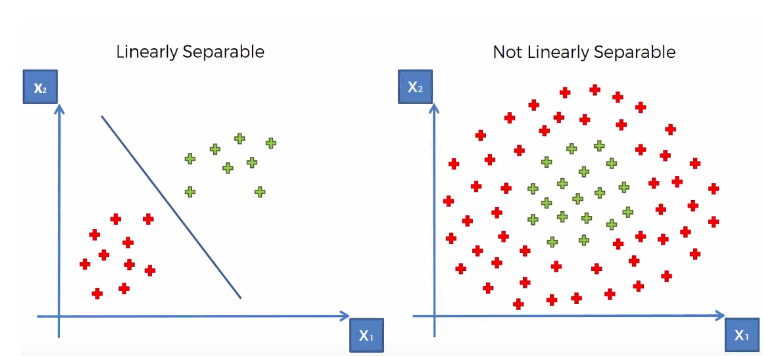
\includegraphics[scale=0.5]{notlinearly.png}} \\

Στην παραπάνω εικόνα παρατηρούμε ότι στην πρώτη περίπτωση τα αντικείμενα μπορούν να διαχωριστούν γραμμικά επιτυχώς, ενώ στη δεύτερη περίπτωση όχι. \\

Ένας πιο αυστηρός ορισμός για τον γραμμικό διαχωρισμό είναι ο εξής: \\
Δύο set αντικειμένων \( K \subseteq \R^{n} \) και \( Ν \subseteq \R^{n} \) είναι γραμμικά διαχωρίσιμα αν \( \exists a \in \R^{n}, b \in \R \) : \(K \subseteq \{ x \in \R^{n} : a^{T} \cdot x \geq b \} \) και \( N \subseteq \{ x \in \R^{n} : a^{T} \cdot x < b\} \). \\



Ένας linear classifier εκπαιδεύεται αρχικά με τα ήδη υπάρχοντα αντικείμενα κι έπειτα για κάθε νέο αντικείμενο αποφασίζει σε ποια από τις δύο ομάδες ανήκει. Πιο αναλυτικά, κατασκευάζεται κατάλληλο hyperplane τέτοιο ώστε τα αντικείμενα της ομαδας Α να βρίσκονται εξ ολοκλήρου από τη μία πλευρά και τα αντικείμενα της ομάδας Β από την άλλη. \\

Στόχος, λοιπόν, είναι να βρεθεί μία γραμμική συνάρτητη f τέτοια ώστε 
\centered{ f(K^{i}) \geq 0 \mbox{ για την ομάδα Α} } 
και
\centered{ f(Ν^{i}) < 0 \mbox{ για την ομάδα Β} }  
όπου f ορίζεται ως \( f(\vec{x}) = a_{1} \cdot x_{1} + a_{2} \cdot x_{2}  + ... + a_{n} \cdot x_{n} \). \\

Το παραπάνω μπορεί να οριστεί και ως πρόβλημα γραμμικού προγραμματισμού: \\
αν y είναι το περιθώριο μεταξύ του αντικειμένου \( K^{i}\) που βρίσκεται πιο κοντά στα αντικείμενα της ομάδας Β και του αντικειμένου \( Ν^{j}\) που βρίσκεται πιο κοντά στα αντικείμενα της ομάδας Α, σκοπός είναι να μεγιστοποιήσουμε το περιθώριο αυτό. Άρα

\centered{\mbox{max y} }
υπό τις προυποθέσεις: \\
\centered{ a_{1} \cdot k_{1} + a_{2} \cdot k_{2}  + ... + a_{n} \cdot k_{n} + b - y \geq 0 \mbox{ για τα αντικείμενα της ομάδας Α} }  
\centered{ a_{1} \cdot n_{1} + a_{2} \cdot n_{2}  + ... + a_{n} \cdot n_{n} + b + y \leq 0 \mbox{ για τα αντικείμενα της ομάδας Β} }  

 
\end{document}
